\documentclass[11pt, a4paper, reqno]{scrartcl}

\usepackage[utf8]{inputenc}
\usepackage{a4wide}
\usepackage{libertine}
\usepackage{graphicx}
\usepackage{listings}
\usepackage{xcolor}
\usepackage{float}
\usepackage{amsmath}

% for latex output of pandas
\usepackage{booktabs}

\begin{document}
    \title{Exercise No. 2}
    \author{David Bubeck, Pascal Becht, Patrick Nisbl\`e}
    \maketitle
    
    \lstset{
        language=Python,
        backgroundcolor=\color{gray!10},
        numbers=left,
        captionpos=t,
        breaklines=true,
        frame=l,
        xleftmargin=\parindent,
        basicstyle=\footnotesize\sffamily,
        keywordstyle=\bfseries\color{green!40!black},
        commentstyle=\itshape\color{purple!40!black},
        identifierstyle=\color{blue!60!black},
        stringstyle=\color{orange}
    }

    \newpage
    \section*{2 - Error analysis of the Euler scheme}

    	\subsection*{a)}
			At first we write the code for the 2 - body problem by using the 
			forward Euler algorithm. We integrate the problem for one orbit and 
			plot it on a double - logarithmic scale. The error will be plotted 
			as a function of $\Delta t$. Therefore we will be using three 
			different eccentricities and various different time steps.
			\newline
			
			Function that integrates the 2 - body problem using the forward 
			Euler algorithm.
			
    		\begin{figure}[H]
        		\lstinputlisting[language=Python,
        			caption={Exercise02a.py},
        			lastline=27]{Exercise02a.py}        
    		\end{figure}
    		
    		
    		Now we plot a circular orbit with the error in energy in a 
    		additional plot. The values that were used are given in the code.
    		
    		\begin{figure}[H]
        		\lstinputlisting[language=Python,
        			caption={Exercise02a.py},
        			firstnumber=30, firstline=30,
        			lastline=51]{Exercise02a.py}   
    		\end{figure}
    		
    		\begin{figure}[H]
    			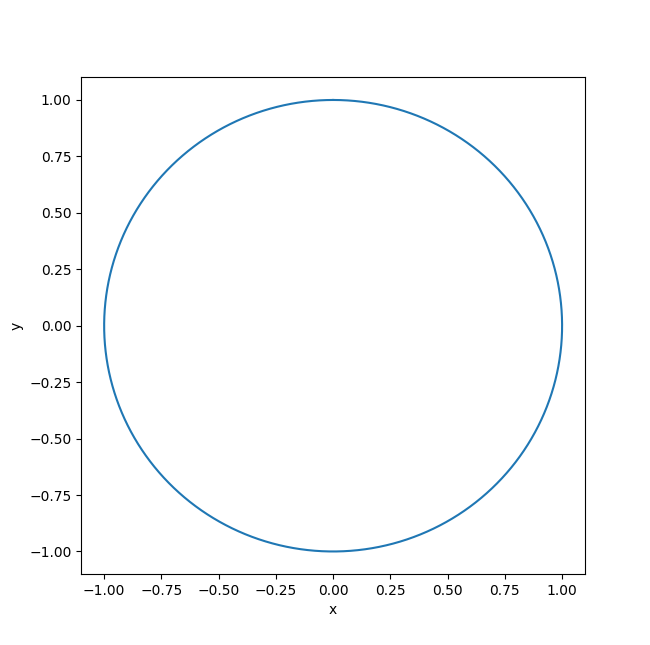
\includegraphics[width=.5\paperwidth]{figure_1.png}
    			\caption{First orbit with forward Euler algorithm}
    		\end{figure}
    		
    		\begin{figure}[H]
    			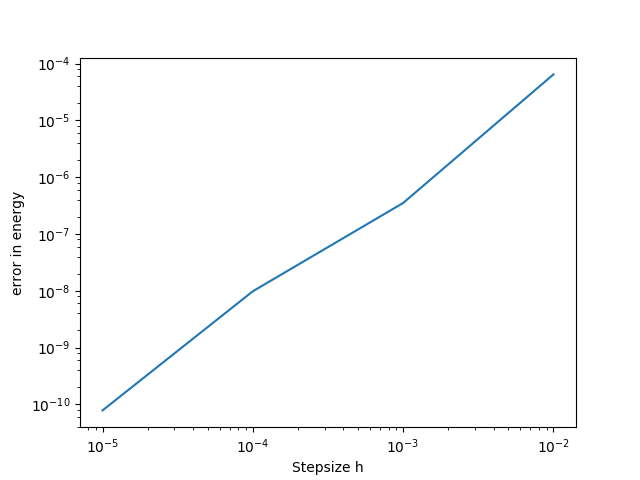
\includegraphics[width=.5\paperwidth]{figure_1_2.png}
    			\caption{First orbit energy error with forward Euler algorithm}
    		\end{figure}
    		
    		
    		We repeat the calculation for two more different initial velocities.
    		
    		For the second orbit we chose:
    		\begin{figure}[H]
        		\lstinputlisting[language=Python,
        			caption={Exercise02a.py},
        			firstnumber=54, firstline=54,
        			lastline=74]{Exercise02a.py}   
    		\end{figure}
    		
    		\begin{figure}[H]
    			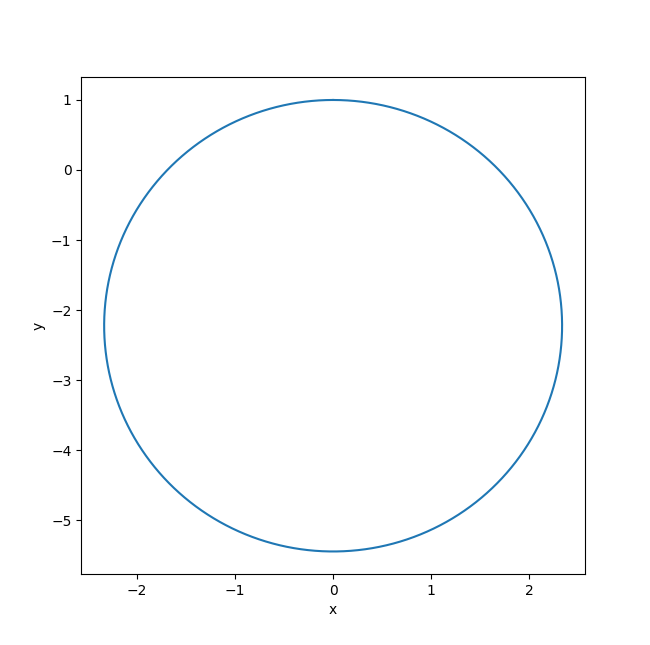
\includegraphics[width=.5\paperwidth]{figure_2.png}
    			\caption{Second orbit with forward Euler algorithm}
    		\end{figure}
    		
    		\begin{figure}[H]
    			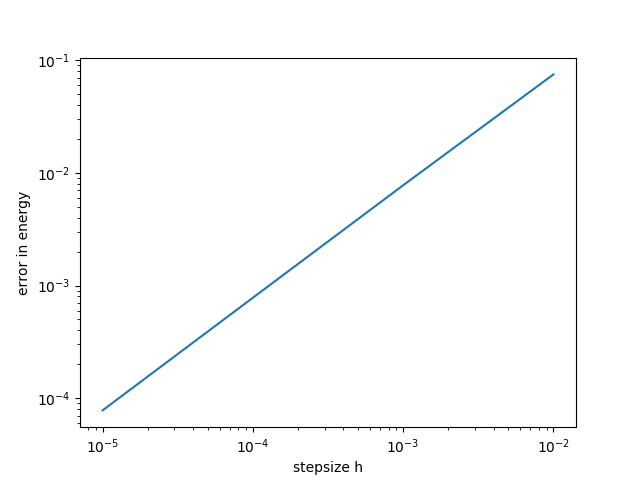
\includegraphics[width=.5\paperwidth]{figure_2_2.png}
    			\caption{Second orbit energy error with forward Euler algorithm}
    		\end{figure}
    		
    		For the third orbit we chose:
    		\begin{figure}[H]
        		\lstinputlisting[language=Python,
        			caption={Exercise02a.py},
        			firstnumber=77, firstline=77,
        			lastline=97]{Exercise02a.py}   
    		\end{figure}
    		
    		\begin{figure}[H]
    			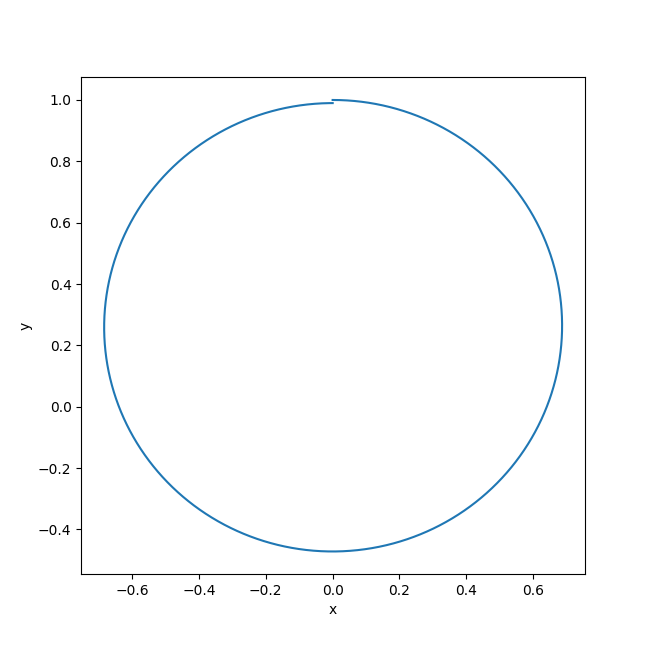
\includegraphics[width=.5\paperwidth]{figure_3.png}
    			\caption{Third orbit with forward Euler algorithm}
    		\end{figure}
    		
    		\begin{figure}[H]
    			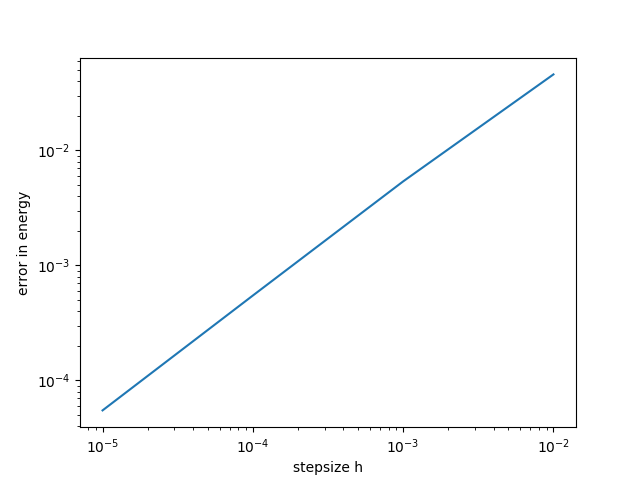
\includegraphics[width=.5\paperwidth]{figure_3_2.png}
    			\caption{Third orbit energy error with forward Euler algorithm}
    		\end{figure}
    		
    	\newpage
    		
    	\subsection*{b)}
			Now we write the code for the 2 - body problem by using the 
			Leapfrog algorithm. We integrate the problem for one orbit and 
			plot it on a double - logarithmic scale. The error will be plotted 
			as a function of $\Delta t$. Therefore we will be using three 
			different eccentricities and various different time steps.
			\newline
			
			Function that integrates the 2 - body problem using the Leapfrog 
			algorithm.
			
    		\begin{figure}[H]
        		\lstinputlisting[language=Python,
        			caption={Exercise02b.py},
        			lastline=31]{Exercise02b.py}        
    		\end{figure}
    		
    		
    		Now we plot a circular orbit with the error in energy in a 
    		additional plot. The values that were used are given in the code. To 
    		be precise we going to use the same values as before.
    		
    		\begin{figure}[H]
        		\lstinputlisting[language=Python,
        			caption={Exercise02b.py},
        			firstnumber=34, firstline=34,
        			lastline=55]{Exercise02b.py}   
    		\end{figure}
    		
    		\begin{figure}[H]
    			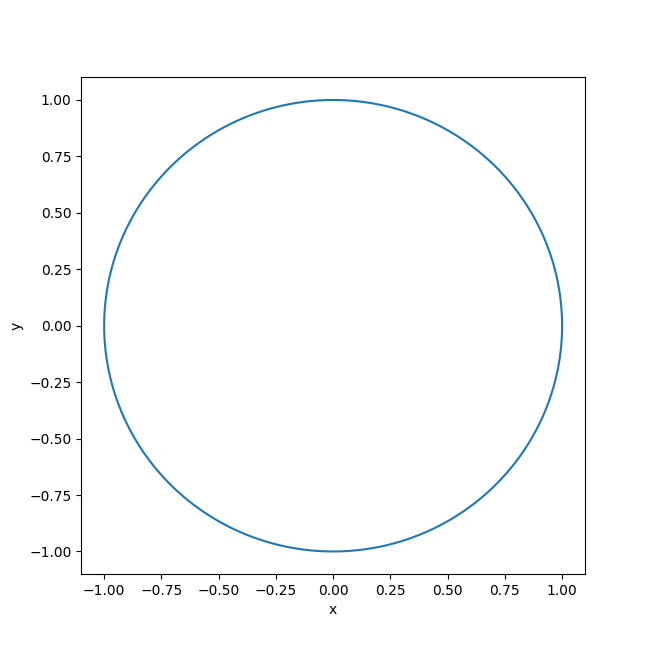
\includegraphics[width=.5\paperwidth]{figure_leap_1.png}
    			\caption{First orbit with leapfrog algorithm}
    		\end{figure}
    		
    		\begin{figure}[H]
    			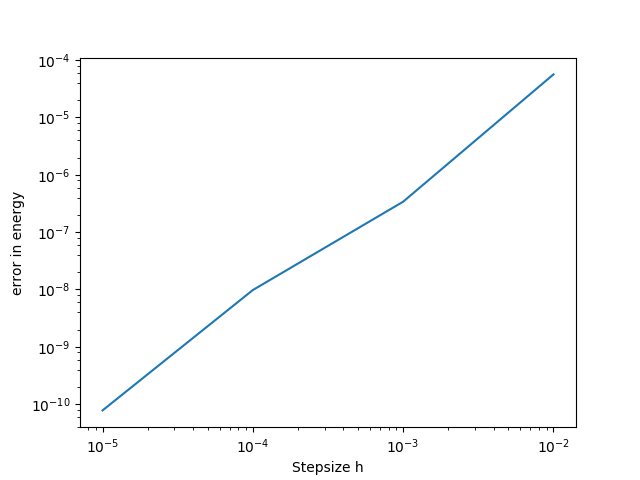
\includegraphics[width=.5\paperwidth]{figure_leap_1_2.png}
    			\caption{First orbit energy error with leapfrog algorithm}
    		\end{figure}
    		
    		
    		We repeat the calculation for two more different initial velocities.
    		
    		For the second orbit we chose:
    		\begin{figure}[H]
        		\lstinputlisting[language=Python,
        			caption={Exercise02b.py},
        			firstnumber=58, firstline=58,
        			lastline=78]{Exercise02b.py}   
    		\end{figure}
    		
    		\begin{figure}[H]
    			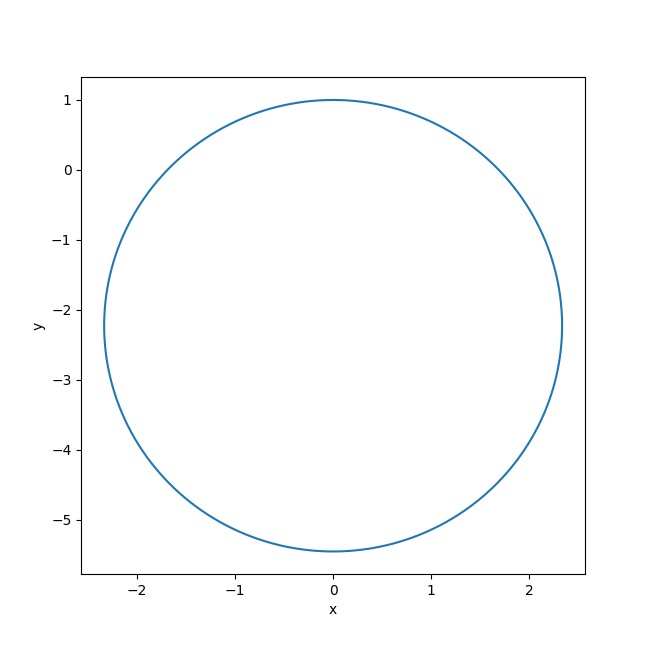
\includegraphics[width=.5\paperwidth]{figure_leap_2.png}
    			\caption{Second orbit with leapfrog algorithm}
    		\end{figure}
    		
    		\begin{figure}[H]
    			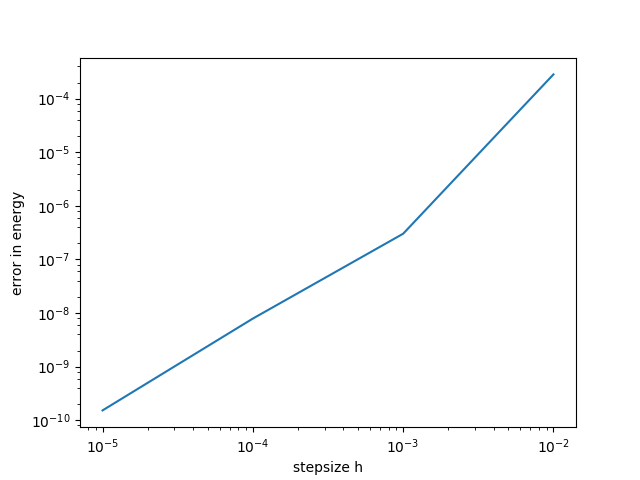
\includegraphics[width=.5\paperwidth]{figure_leap_2_2.png}
    			\caption{Second orbit energy error with leapfrog algorithm}
    		\end{figure}
    		
    		For the third orbit we chose:
    		\begin{figure}[H]
        		\lstinputlisting[language=Python,
        			caption={Exercise02b.py},
        			firstnumber=81, firstline=81,
        			lastline=101]{Exercise02b.py}   
    		\end{figure}
    		
    		\begin{figure}[H]
    			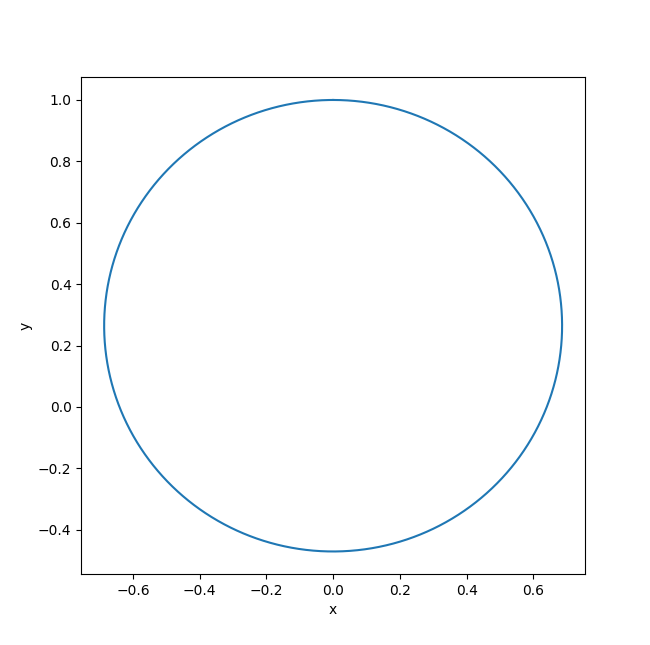
\includegraphics[width=.5\paperwidth]{figure_leap_3.png}
    			\caption{Third orbit with leapfrog algorithm}
    		\end{figure}
    		
    		\begin{figure}[H]
    			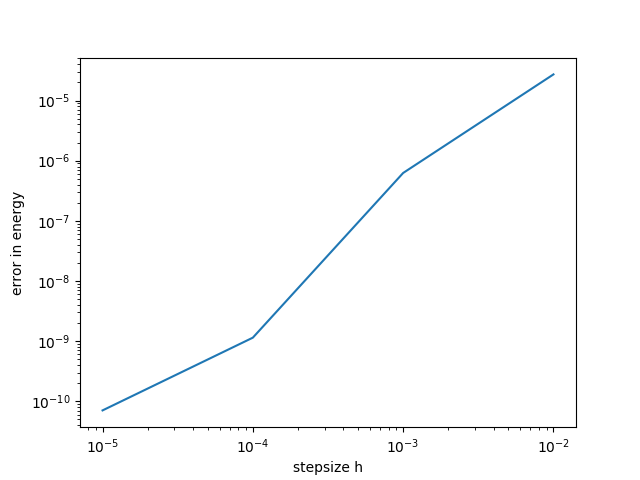
\includegraphics[width=.5\paperwidth]{figure_leap_3_2.png}
    			\caption{Third orbit energy error with leapfrog algorithm}
    		\end{figure}
    		
    		
    		The errors decreas with decreasing time steps for both integration 
    		schemes. For the euler algorithm we expect a decreasing with $O(h^2)
    		$, for the Leapfrog algorithm $O(h^3)$. This is what we get. The 
    		errors of the Leapfrog integration are much smaller than those of 
    		the Euler integration. However, the slope of the errorr - curve is 
    		steeper which we also expect. Another difference between the error - 
    		plots, of the two integration variations, is, that for the Euler 
    		integration we get straight lines whereas for the Leapfrog 
    		integration the errors seem to scatter around the expected line. 

\end{document}